\renewcommand{\theequation}{\theenumi}
\begin{enumerate}[label=\thesection.\arabic*.,ref=\thesection.\theenumi]
\numberwithin{equation}{enumi}

\item Join CD as shown in the figure \ref{fig:intersecting_chords}
\begin{figure}[!ht]
\centering
\resizebox{\columnwidth}{!}{%Exercise 8.1 prob 47
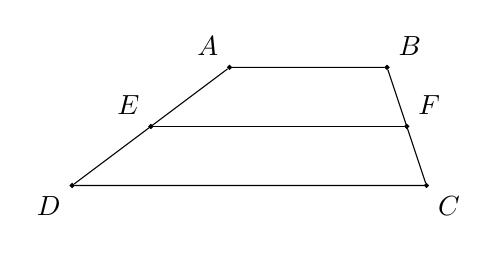
\begin{tikzpicture}
[scale=0.5,>=stealth,point/.style={draw,circle,fill = black,inner sep=0.5pt},]
%\tikzset{shift={(-3,0)}}
%Triangle sides
\def\a{4}
\def\c{9}
\def\d{5}
\def\h{3}
\def\k{1.5}
%\def\c{7.5}

%Labeling points
\node (D) at (0,0)[point,label=below left:$D$] {};
\node (B) at (8,\h )[point,label=above right:$B$] {};
\node (C) at (\c, 0)[point,label=below right:$C$] {};
\node (E) at (2, \k)[point,label=above left:$E$] {};
\node (F) at (8.5, \k)[point,label=above right:$F$] {};
%\node (M) at (4, \k)[point,label=below right:$M$] {};
%\node (N) at (8, \k)[point,label=below right:$N$] {};
%\node (X) at (4, 0)[point,label=below right:$X$] {};
%%node (Y) at (8, 0)[point,label=below right:$Y$] {};
\node (A) at (4,\h)[point,label=above left:$A$] {};
%A



%Drawing parallelogram ABCD
\draw (A) -- (B) --  (C) --(D)--(A);
\draw (E) --(F);
%\draw (B) --(Y);



%
\end{tikzpicture}

}
\caption{Chords of the circle intersecting at point B by Latex-Tikz}
\label{fig:intersecting_chords}	
\end{figure}

\item Show that angle subtended by a chord at the centre is twice the angle subtended by it at any point on the circumference
%figure for proof
\begin{figure}[!ht]
\centering
\resizebox{\columnwidth}{!}{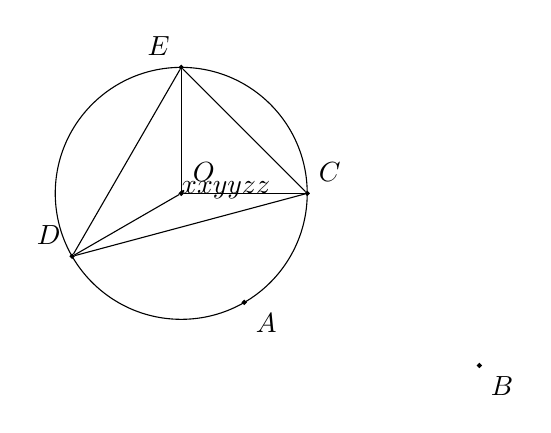
\begin{tikzpicture}
[scale=0.4,>=stealth,point/.style={draw,circle,fill = black,inner sep=0.5pt},]
%\tikzset{shift={(-3,0)}}

%innput parameters
\def\r{4}

%Labeling points
% r sin(pi/3) = 3.4641
\node (O) at (0,0)[point,label=above right:$O$] {};
\node (C) at (\r, 0 )[point,label=above right:$C$] {};
\node (A) at ({\r/2},-3.4641)[point,label=below right:$A$] {};
\node (D) at (-3.4641 , -{\r/2})[point,label=above left:$D$] {};
\node (E) at (0 , \r)[point,label=above left:$E$] {};
\node (B) at (9.4641 , -5.4641)[point,label=below right:$B$] {};


%A



%Drawing parallelogram ABCD
%\draw (O) -- (A);
\draw (O) -- (C);
\draw (O) -- (E);

\draw (E) -- (D);
\draw (D) -- (C);
\draw (E) -- (C);
\draw (O) -- (D);
%\draw (D) -- (B);
%\draw (E) -- (B);


\draw (O) circle (\r);
%marking angles
%\tkzMarkAngle[fill=orange!0.5,size=0.003cm,mark=](C,D,O)
%\tkzMarkAngle[fill=green!60,size=0.003cm,mark=](O,C,D)
%\tkzMarkAngle[fill=green!0.5,mark=](O,D,E)
%\tkzMarkAngle[fill=green!0.5,mark=](D,E,O)
%\tkzMarkAngle[fill=green!0.5,mark=](O,E,C)
%\tkzMarkAngle[fill=green!0.5,mark=](E,C,O)
\tkzLabelAngle[pos=1.90](C,D,O){$x$}
\tkzLabelAngle[pos=1.90](O,C,D){$x$}
\tkzLabelAngle[pos=1.30](O,D,E){$y$}
\tkzLabelAngle[pos=1.30](D,E,O){$y$}
\tkzLabelAngle[pos=1.00](O,E,C){$z$}
\tkzLabelAngle[pos=1.00](E,C,O){$z$}

%
\end{tikzpicture}
}
\caption{Angles subtended by chord ED at centre O and point C by Latex-Tikz}
\label{fig:chord_proof}	
\end{figure}
\newline
Solution:
\newline
In the figure \ref{fig:chord_proof}	
\begin{align}
OC = OD = OE = r
\end{align}
$\triangle DOE, \triangle DOC, \triangle COE$ are isosceles triangles.
\newline
Hence their base angles are equal as indicated in figure \ref{fig:chord_proof}

\item In $\triangle EDC$ in figure \ref{fig:chord_proof} , We know sum of the angles in a triangle is $180^{\circ}$
\begin{align}
2(x+y+z) = 180^{\circ}
\\
180^{\circ} - 2y = 2(x+z)
\label{eq:val2y}
\end{align}

\item In $\triangle EOD$ in figure \ref{fig:chord_proof} as sum of the angles in a triangle is $180^{\circ}$,
\begin{align}
\angle EOD = 180^{\circ} - 2y
\label{eq:angle1proof}
\end{align}
Substituting equation \ref{eq:val2y} in equation \ref{eq:angle1proof} we get 
\begin{align}
\angle EOD = 2(x+z)
\\
\angle EOD = 2 \angle ECD
\\
\angle ECD = \frac{\angle EOD}{2} = \frac{\alpha}{2}
\label{eq:angle1}
\end{align}
Hence angle subtended by the chord at the centre is twice the angle subtended by it at a point on the circumference.

\item From \ref{fig:intersecting_chords} AC subtends $\angle AOC = \beta$ at the centre and $\angle ADC$ at the circumference.
\begin{align}
\implies \angle ADC = \frac{\angle AOC}{2}
\\
\implies \angle ADC = \frac{\beta}{2}
\label{eq:angle2}
\end{align}


\item In $\triangle DBC$ from \ref{eq:angle1} and \ref{eq:angle2}
\begin{align}
\angle BCD = 180^{\circ} - \angle ECD
\\
\angle BCD = 180^{\circ} - \frac{\alpha}{2}
\label{eq:tri1}
\\
\angle BDC = \angle ADC = \frac{\beta}{2}
\label{eq:tri2}
\\
\angle CBD = \angle CBA = \theta
\label{eq:tri3}
\end{align}

Sum of the angles in a triangle is $180^{\circ}$. So In $\triangle DBC$
\begin{align}
\angle CBD + \angle BDC + \angle BCD = 180^{\circ}
\label{eq:trisum}
\end{align}
Substituting equations \ref{eq:tri3},\ref{eq:tri3},\ref{eq:tri3} in \ref{eq:trisum}
\begin{align}
\theta + \frac{\beta}{2} + 180^{\circ} - \frac{\alpha}{2} = 180^{\circ}
\\
\theta = \frac{\alpha}{2} - \frac{\beta}{2}
\\
\theta = \frac{\alpha - \beta}{2} 
\end{align}
Hence proved.
\end{enumerate}
